\chapter{Trasformata di Hilbert} 

\begin{figure}[h]
    \centering
    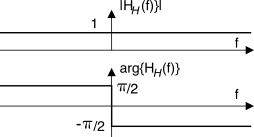
\includegraphics[scale = 2]{Filtro di Hilbert.png}
\end{figure}  

\newpage 

\section{Cosa è la trasformata di Hilbert} 

La trasformata di Hilbert è una particolare rappresentazione, che, contrariamente ad altre trasformate 
non realizza un cambiamento del dominio di definizione. \newline 

In altre parole, a partire da una funzione del tempo s(t), la trasformata di Hilbert $s^{\sim} (t)$ è ancora una funzione del tempo. \newline 

$s^{\sim} (t)$ si ottiene come uscita da un filtro, detto filtro di Hilbert, caratterizzato dalla funzione di trasferimento: 

{
    \Large 
    \begin{equation}
        H_H (f) = 
        \begin{cases}
            -\jmath \text{ per } f>0  \\ 
            0 \text{ per } f = 0 \\ 
            \jmath \text{ per } f<0
        \end{cases}
    \end{equation}
}

in termini di parte reale e parte immaginaria, avremo: 

{
    \Large 
    \begin{equation}
        \abs{H_H (f)} = 
        \begin{cases}
            1 \text{ per } f \neq 0 \\ 
            0 \text{ per } f = 0
        \end{cases}
    \end{equation}
}

{
    \Large 
    \begin{equation}
        \arg{H_H (f)} = 
        \begin{cases}
            -\frac{\pi}{2} \text{ per } f > 0 \\ 
            0 \text{ per } f = 0 \\ 
            \frac{\pi}{2} \text{ per } f < 0
        \end{cases}
    \end{equation}
}

in termini di parte reale e fase. \newline 

Schematizzando i filtri ed i segnali, avremo che: 

\begin{figure}[h]
    \centering
    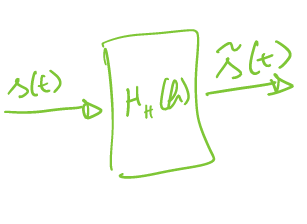
\includegraphics[scale = 0.5]{trasformata di Hilbert segnali con filtro.PNG}
\end{figure} 

Nel dominio della frequenza, si ha: 

{
    \Large 
    \begin{equation}
        S^{\sim} (f) = H_H (f)S(f)
    \end{equation}
}

dove $S(f)$ è la trasformata di Fourier di s(t) mentre $S^{\sim}(f)$ è la trasformata di Fourier di $s^{\sim} (t)$. \newline 

Sapendo la relazione tra frequenza e tempo, possiamo sapere che la risposta impulsiva del filtro di Hilbert nel tempo è: 

{
    \Large 
    \begin{equation}
        h_H (t) = \frac{1}{\pi t}
    \end{equation}
}

Grazie alle proprietà della trasformata di Fouerier, sapendo che $H_H (f)$ è una funzione puramente immaginaria e dispari, 
anche $h_H (t)$ è puramente reale e dispari. \newline 

L'operazione di trasformazione inversa di Hilbert, che consente di riottenere il segnale s(t) a partire da $s^{\sim} (t)$ richiede, in realtà, una nuova trasformata di Hilbert:

{
    \Large 
    \begin{equation}
        \begin{split}
            S^{\approx} 
            &= 
            H_H(f) S^{\sim} (f) 
            \\ 
            &= 
            H_H(f) H_H(f) S(f) 
            \\ 
            &= 
            -S(f)
        \end{split}
    \end{equation}
}

Questa relazione vale per tutti i valori $f \neq 0$. \newline 

In $f=0$, il valore $S(0)$, se diverso da zero, viene annullato, e non potrà essere più recuperato. \newline 

In particolare, se il segnale ha valore medio diverso da zero, questo si tradurrebbe nella presenzza nello spettro di una delta di Dirac posizionata nell'origine. \newline 

Di conseguenza, possiamo concludere che la classe dei segnali per cui è applicabile la trasformata di Hilbert è quella dei segnali a valor medio nullo. \newline 

Dal punto di vista ingegneristico: 

\begin{figure}[h]
    \centering
    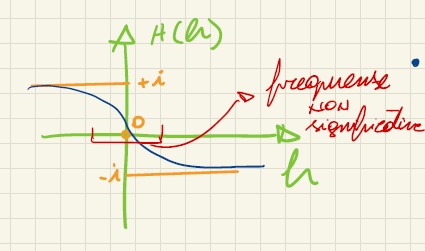
\includegraphics[scale = 0.5]{Considerazioni filtro di Hilbert in frequenza.PNG}
\end{figure}  

inoltre, è difficilmente realizzabile un filtro con una transizione così brusca, quindi, 
generalmente, la transizione è "smussata". \newline 

\newpage